\chapter{Introduction}\label{chap:intro}

This chapter introduces the research problem by examining the security challenges associated with smart-home communication networks, with particular emphasis on the ECHONET Lite protocol and its application in residential energy management. Section 1.1 provides an overview of the evolution of the Smart Grid, Home Energy Management Systems (HEMS), and Machine-to-Machine (M2M) communication in residential environments, highlighting the associated cybersecurity concerns. Section 1.2 presents an overview of the ECHONET Lite protocol, including its communication model, frame structure, and limitations in providing native application-layer security. Section 1.3 examines the cybersecurity threats affecting smart-home networks, including device compromise, replay attacks, message injection, and denial-of-service attacks, and discusses their implications for information security, device operation, and residential energy management. Section 1.4 explains the motivation for this research, focusing on the need for a lightweight security mechanism suitable for ECHONET Lite communication. Section 1.5 defines the research problem concerning the absence of built-in message authentication, integrity verification, and anti-replay protection in standard ECHONET Lite frames. Section 1.6 presents the research objectives, while Section 1.7 establishes the scope and limitations of the study. Section 1.8 outlines the intended research contributions, and Section 1.9 describes the five stages of the research process, from threat analysis and mechanism design to implementation, evaluation, and analysis of results. Finally, Section 1.10 outlines the organization of the remaining chapters of the thesis.

% This chapter, divided into thirteen sections, introduces the research problem and situates it within the broader evolution of residential energy management and smart home communication security. Section 1.1 traces the transition from centralized Smart Grid infrastructure to Machine-to-Machine (M2M) enabled smart home networks and classifies domestic communication protocols across the OSI model. Section 1.2 presents a detailed technical overview of the ECHONET Lite protocol, its frame structure, and its native security posture. Section 1.3 analyzes the cybersecurity threat landscape confronting smart home networks and taxonomizes the principal attack vectors relevant to this study. Sections 1.4 and 1.5 articulate the research motivation and problem statement, respectively, Section 1.6 enumerates the research objectives, and Section 1.7 defines the scope, boundaries, and underlying assumptions of the study. Section 1.8 discusses the theoretical and practical contributions of this thesis, and Section 1.9 outlines the five-phase research roadmap adopted to achieve the stated objectives. Section 1.10 presents the organization of the remaining chapters, Section 1.11 discusses the academic and industrial significance of the study, Section 1.12 defines key terms used throughout the thesis, and Section 1.13 closes the chapter with a concise summary.


\section{Overview}

The twenty-first century has ushered in a profound reimagining of how electricity is generated, distributed, and consumed, as the global energy ecosystem pivots decisively from rigid, centralized power networks toward the intelligent, data-driven architecture of the Smart Grid. Driven by national decarbonization goals, fluctuating energy costs, and the need for peak-load balancing, traditional centralized generation networks are being replaced by automated Demand-Side Management (DSM) architectures. Within this ecosystem, Home Energy Management Systems (HEMS) serve as the primary coordination hubs connecting the utility grid to the residential domain, dynamically optimizing household power consumption by interacting directly with distributed energy resources (DERs) such as solar inverters, electric vehicle (EV) chargers, battery storage units, and major residential appliances.
Historically, electricity distribution followed a strictly unidirectional model, in which bulk power was generated at centralized plants, stepped up for transmission, and delivered to passive residential consumers with no feedback path other than periodic metering. The Smart Grid paradigm inverts this relationship by embedding bidirectional communication, distributed sensing, and automated control throughout the distribution network, allowing utilities and consumers to jointly participate in load balancing, dynamic pricing response, and renewable energy integration. As distributed generation and storage assets have proliferated at the household level, the locus of intelligent control has progressively shifted from the utility substation to the consumer premises, giving rise to HEMS as the residential counterpart of utility-scale Energy Management Systems (EMS). This evolutionary trajectory, from centralized generation to distributed, consumer-centric orchestration, forms the structural backdrop against which the communication processes binding HEMS to household devices, and the security implications that follow from them, must be understood.
Realizing this residential intelligence, however, is not a matter of software alone. It depends on a dense fabric of Machine-to-Machine (M2M) communication protocols that allow a HEMS controller to discover, query, and command a heterogeneous population of edge devices. Residential devices are no longer passive electrical loads, since they now operate as autonomous, energy-aware nodes capable of real-time telemetry reporting and automated load shedding, and no single protocol dominates the task of connecting them. Zigbee, Z-Wave, Bluetooth Low Energy, Wi-Fi based transports, and the more recent Matter standard coexist across markets, while in Japan, one of the most mature HEMS deployment environments globally, ECHONET Lite, standardized by the ECHONET Consortium since 1997, serves as the de facto application layer protocol binding smart meters, solar inverters, storage batteries, and over 120 classes of appliances into a single interoperable ecosystem (ECHONET Consortium, 2026). Unlike enterprise or industrial M2M deployments, which typically operate within professionally managed and monitored network perimeters, these domestic M2M ecosystems are provisioned, configured, and maintained largely by non-expert end users, over consumer grade routers, and alongside untrusted general-purpose devices sharing the same local area network. This distinction is significant from a security standpoint, since the same properties that make smart home M2M networks convenient and low cost, namely plug-and-play discovery, minimal configuration overhead, and lightweight messaging, also reduce the opportunity for the centralized security governance that is typical of enterprise or industrial control networks.
However, the hyper-connectivity of domestic M2M networks significantly expands the residential attack surface. Compromised local networks or rogue edge nodes introduce severe operational threats, as malicious command injection can disrupt device operations or cause artificial power spikes across local distribution networks. Protecting application layer messaging within smart home environments is therefore essential to preserving consumer privacy, physical asset integrity, and grid reliability. Because HEMS gateways aggregate telemetry from, and issue control commands to, multiple appliances simultaneously, a single compromised message exchange can cascade into coordinated, multi-device disruption, an effect that has no direct analogue in traditional single-appliance fault scenarios.
The urgency of securing residential M2M messaging is not speculative, since it is grounded in a well-documented and rapidly worsening global cyber-threat trajectory. Cybersecurity Ventures estimated that worldwide cybercrime losses grew from approximately USD 3 trillion in 2015 to USD 6 trillion in 2021, and forecast that damages would reach USD 10.5 trillion annually by 2025, a growth rate of roughly 15 percent per year that would make cybercrime, if measured as an economy, larger than that of most nations (Morgan, 2020).

% \TODO{Table 1.0: Growth Trajectory of Global Cybercrime Costs}
\begin{table}[htbp]
  \centering
  \caption{Security consequences associated with insecure connected devices and networks}
  \label{tab:security_consequences_intro}
  \renewcommand{\arraystretch}{1.2}
  \begin{tabular}{p{3.2cm} p{5.2cm} p{5.2cm}}
    \hline
    \textbf{Security Concern}                                                                              & \textbf{Observed Consequence} & \textbf{Relevance to Residential M2M Systems} \\
    \hline

    Weak authentication                                                                                    &
    Unauthorized access, device takeover, and data exposure                                                &
    Demonstrates the consequences of insufficient authentication mechanisms in connected residential devices.                                                                              \\

    Insecure smart-home devices                                                                            &
    Privacy violations, unauthorized control, malware, and denial-of-service (DoS) attacks                 &
    Highlights the security risks associated with network-connected household devices.                                                                                                     \\

    Compromised IoT devices                                                                                &
    Recruitment into botnets and participation in large-scale distributed denial-of-service (DDoS) attacks &
    Shows how vulnerable residential devices can contribute to attacks beyond the local network.                                                                                           \\

    Insecure communication                                                                                 &
    Message spoofing, unauthorized commands, and manipulation of device operations                         &
    Directly relates to the need for protecting M2M messages exchanged between HEMS and residential devices.                                                                               \\

    Cybersecurity incidents                                                                                &
    Financial losses, service disruption, and operational damage                                           &
    Establishes the broader economic and operational significance of cybersecurity weaknesses.                                                                                             \\

    Insecure cyber-physical systems                                                                        &
    Potential safety, reliability, and physical consequences following unauthorized control                &
    Demonstrates why communication security is important when networked devices influence physical processes.                                                                              \\

    \hline
  \end{tabular}
\end{table}

% add ref later %\ref{tab:security_consequences_intro}
The reported consequences of security weaknesses across connected devices and cyber-physical environments can be summarized as shown in Table~Chapter-2. A more comprehensive synthesis of the supporting literature is presented in Chapter~2.

Beyond these aggregate projections, documented incidents quantify what under secured, network-connected consumer devices are capable of producing in practice. Botnets assembled from compromised IoT devices, typically hijacked through factory default or weak credentials, have been used to launch distributed denial of service (DDoS) attacks of escalating scale, with recorded peaks including a 620 Gbit/s attack in 2016 and, most recently, a 31.4 Tbps attack in 2024, each generated by networks of hundreds of thousands of compromised consumer grade devices (Antonakakis et al., 2017). Beyond raw attack bandwidth, these campaigns have produced concrete financial and operational damage, as affected organizations have reported direct incident response costs in the hundreds of thousands of dollars, follow-on cybersecurity budget increases exceeding a million dollars, and outages that rendered major internet services inaccessible across entire regions (Antonakakis et al., 2017; Fruhlinger, 2018). Beyond large-scale denial of service, the same class of unauthenticated, under secured consumer devices is equally susceptible to more targeted forms of abuse, including unauthorized command injection, message spoofing, and replay attacks, none of which require assembling a botnet at all, but merely require an attacker to reach a device that cannot verify who is instructing it. These figures and attack categories demonstrate, in concrete financial and operational terms, the class of damage that under secured, M2M connected consumer devices are capable of producing, the same class of device, protocol, and deployment context that this study is concerned with.
This risk is not distributed evenly across the protocol landscape introduced earlier in this section, since it is a direct function of protocol design. Some ecosystems build device identity and transport layer encryption into their core specification, while others defer security entirely to whatever network boundary happens to surround them. ECHONET Lite falls unambiguously into the latter category, and it is for this reason that the protocol is the specific focus of this study rather than the smart home M2M landscape in general. Its specification deliberately confines itself to interoperability concerns, such as device object modeling, command semantics, and vendor neutral control sequences, while leaving authentication, encryption, and message integrity entirely outside its scope. This is not a latent or theoretical weakness. It is openly acknowledged by engineers working directly with the protocol, who note plainly that ECHONET Lite communications involve no authentication and no encryption whatsoever, and that any host able to reach a device's listening port, conventionally UDP port 3610, can issue control commands to it, with safe operation depending entirely on external network containment rather than on the protocol itself. Tellingly, this gap persists at the standards body level even today, since only in 2026 did the ECHONET Consortium begin incorporating PKI based identity and authentication services through a new industry partnership with SEALSQ Corp, nearly three decades after the protocol's initial standardization and long after its mass deployment across residential HEMS installations (ECHONET Consortium, 2026). Wherever ECHONET Lite traffic is secured at all in practice, that security is bolted on externally, through network segmentation, VPN tunneling, or SSL/TLS wrapping at a gateway layer, and never as an intrinsic property of the ECHONET Lite message itself.
Set against the cybercrime trajectory and attack figures documented above, this is not an abstract protocol shortcoming. It is a live instance of the exact failure mode already shown to produce national scale service outages and seven figure institutional costs, now situated at the control plane of an increasingly grid critical residential infrastructure. The broader trend among contemporary smart home protocols has, in fact, moved decisively in the opposite direction from ECHONET Lite's security agnostic design. Zigbee 3.0 mandates AES-128 encryption together with a trust center link key mechanism as a second layer of protection (MDPI, 2025), while Matter, the most recent major interoperability standard, embeds AES-128-CCM encryption, public key infrastructure based device attestation, and certificate based secure commissioning directly into its core specification, so that every device must cryptographically prove its manufacturer identity before it is ever allowed to join a network (ACM Internet Measurement Conference, 2026). Security, in other words, has increasingly become a first class design requirement of modern M2M protocols rather than an afterthought left to perimeter defenses. ECHONET Lite's continued reliance on external, bolted on protections therefore represents not merely a gap but a growing divergence from prevailing protocol design practice. Because HEMS exists specifically to mediate between residential appliances and the broader Smart Grid, scheduling EV charging, dispatching battery storage, and responding to utility price signals, an attacker who can forge or intercept unauthenticated ECHONET Lite messages gains more than access to a single appliance. Such an attacker gains a foothold capable of manipulating the very load balancing and DSM functions that the Smart Grid transition was designed to enable in the first place. Perimeter defenses such as VLANs and VPNs assume a trust boundary that, once crossed, for instance by a compromised device already resident on the same LAN, offers no further resistance, since the protocol itself cannot distinguish a legitimate controller from an impersonating one. It is this precise architectural deficiency, increasingly at odds with where comparable protocols have already moved, that motivates the central objective of this study, which is to enable security natively within ECHONET Lite messaging itself, rather than to continue relying on the ad hoc, externally bolted on protections that have characterized its deployment to date.

\section{ECHONET Lite Protocol: An Overview}


Established by the ECHONET Consortium and recognized under ISO/IEC 14543-4-3, the ECHONET Lite protocol specification defines standard communication for smart home appliances and HEMS devices. Enforced across international markets and widely adopted in residential deployments, ECHONET Lite normalizes multi-vendor interoperability across more than 100 device classes, including HVAC units, smart meters, heat pump water heaters, and photovoltaic arrays.

ECHONET Lite occupies a distinctive position among smart home messaging standards because it was developed specifically with energy management semantics at its core, rather than as a general-purpose IoT messaging layer later adapted for energy use cases. Its object-oriented device model, in which every appliance class exposes a standardized set of properties (e.g., operational status, power consumption, set-point temperature), allows HEMS controllers to interoperate with appliances from different manufacturers without bespoke integration work. This device-class standardization has made ECHONET Lite the de facto messaging backbone for HEMS certification programs in several national smart grid initiatives, embedding it deeply into residential energy policy infrastructure rather than treating it as an optional convenience layer. The protocol's continued longevity, despite the emergence of newer general-purpose smart home standards such as Matter, is attributable to this entrenched role in energy-sector certification and the substantial installed base of already-deployed HEMS-compliant appliances.

\begin{figure}[htb!]
  \centering
  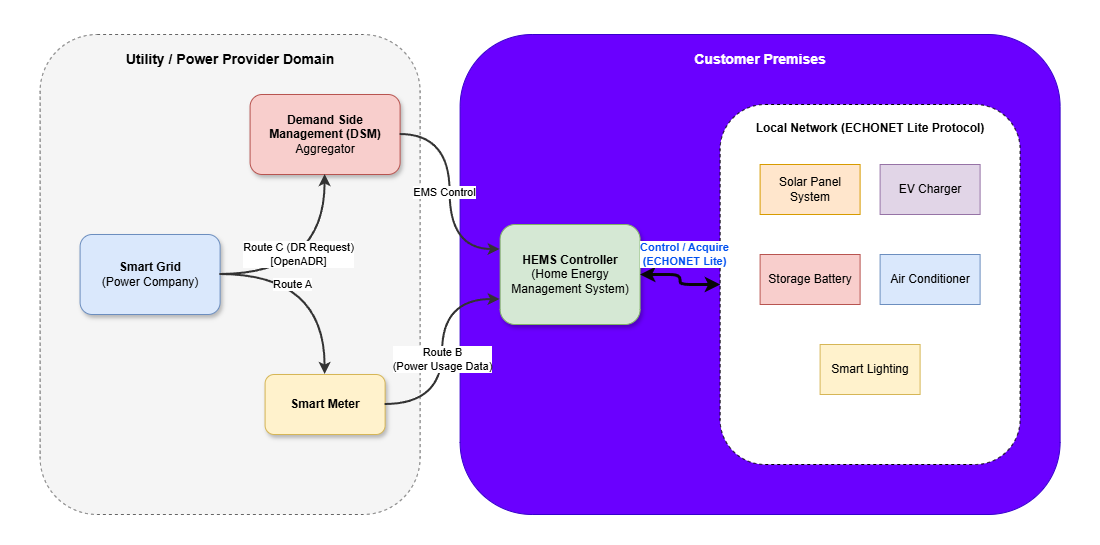
\includegraphics[width=0.85\textwidth]{chapters/figures/Architecture diagram.png}
  \caption{Echonet Lite Architecture.}
  \label{fig:echonet-architecture}
\end{figure}

ECHONET Lite uses an object-property-action model to govern device behavior. Devices send read, write, or notification requests (Get, Set, SNA) over unicast or multicast IP channels. The ESV command code field, in particular, determines the semantic intent of a frame (e.g., `0x62` for a property read request, `0x61` for a property write request, `0x73` for an unsolicited property notification), and it is precisely this field, together with the EDT payload it governs, that an attacker targets when attempting unauthorized command injection or replay. Because the SEOJ/DEOJ addressing scheme identifies devices purely by class and instance codes rather than by any cryptographically verifiable identity, any node capable of observing or injecting traffic on the local network segment can construct a syntactically valid ECHONET Lite frame addressed to any other device on that segment.

Despite its widespread structural adoption, standard ECHONET Lite transmits plaintext binary frames without mandatory application-layer cryptographic encipherment or dynamic origin authentication. Designed originally for physically closed, trusted home networks, native ECHONET Lite frames lack fields for data confidentiality, frame integrity, or sender identity verification. Wrapping ECHONET Lite in heavy lower-layer transport security protocols (such as DTLS or TLS) often introduces excessive processing overhead, memory footprint expansion, and latency spikes on resource-constrained 8-bit or 16-bit appliance microcontrollers. In practice, this leaves implementers with an unappealing binary choice: ship devices with no meaningful application-layer protection, or absorb the disproportionate computational cost of a full transport-security handshake on hardware that was never provisioned with that overhead in mind. This unresolved tension between security completeness and embedded resource constraints is the central technical gap that motivates the present research.


\section{Smart-Home Networks and Cybersecurity Threats}

The increasing adoption of Internet of Things (IoT) technologies has transformed conventional residential environments into interconnected smart-home ecosystems in which sensing, communication, computation, and physical control are increasingly integrated. Unlike traditional household appliances that operated independently, smart-home devices can exchange information with one another, communicate with home gateways and cloud services, and receive commands from users through local or remote interfaces. This connectivity provides significant benefits in terms of convenience, energy management, automation, and remote monitoring; however, it also introduces cybersecurity risks because devices that were previously isolated from communication networks are now exposed to a wider range of digital interactions. Security and privacy have consequently become important considerations in the design and deployment of smart-home systems \citep{haneySmartHomeSecurity2020}.

The security characteristics of smart-home networks differ from those of conventional enterprise networks. Enterprise environments are generally supported by dedicated information-technology personnel, centrally managed security policies, controlled network infrastructure, and continuous monitoring. In contrast, smart-home environments commonly contain heterogeneous devices from multiple manufacturers, consumer-grade network equipment, mobile applications, cloud services, and general-purpose personal devices operating within the same residential environment. Many of these devices are designed with limited computational, storage, and energy resources, which can constrain the implementation of sophisticated security mechanisms. Furthermore, residential users may have limited technical knowledge and may not possess the expertise required to configure and continuously maintain the security of every connected device. Studies of smart-home users have consequently identified a gap between users' awareness of security and privacy risks and their ability to implement effective mitigation measures \citep{haneySmartHomeSecurity2020}.

The increasing number of interconnected devices consequently expands the attack surface of the residential network. A compromise of one device may provide an attacker with an opportunity to interact with other devices or services within the same environment, particularly when network segmentation and access controls are insufficient. This concern extends beyond conventional information security because smart-home devices frequently interact with physical systems. For example, a compromised thermostat, lighting controller, door lock, surveillance camera, energy-management device, or appliance may allow an attacker to alter physical conditions within the residence. In energy-oriented smart homes, the consequences can extend further because Home Energy Management Systems (HEMS) can coordinate multiple appliances and distributed energy resources. Consequently, unauthorized manipulation of a single communication exchange may affect the operation of several interconnected devices simultaneously. The cyber-physical nature of smart-home environments therefore creates security consequences that may involve not only information and privacy but also physical safety, household operations, and energy management \citep{heartfieldTaxonomyCyberphysicalThreats2018}.

Cybersecurity threats against smart-home networks can be considered in relation to the fundamental security requirements of confidentiality, integrity, and availability. Confidentiality concerns the protection of information from unauthorized disclosure, which is particularly important in residential environments because connected devices can generate information capable of revealing household activities, occupancy patterns, energy consumption, and user behaviour. Integrity concerns ensuring that information and commands are not modified by unauthorized parties. This is particularly significant for smart-home control systems because an altered command may cause an appliance to perform an operation that was not requested by the legitimate user. Availability concerns ensuring that legitimate users and devices can access required services when needed. A denial-of-service condition affecting a gateway, controller, or communication channel may therefore prevent legitimate control and monitoring operations. Research on smart-home cyber-physical threats similarly demonstrates that attacks against connected residential systems can produce consequences extending from information disclosure to unauthorized control and physical effects \citep{heartfieldTaxonomyCyberphysicalThreats2018}.

The practical significance of these vulnerabilities has been demonstrated by attacks against consumer IoT devices. One prominent example is the Mirai botnet, which demonstrated how inadequately secured IoT devices could be compromised and collectively used to conduct large-scale distributed denial-of-service (DDoS) attacks \cite{antonakakisUnderstandingMiraiBotnet}.

The Mirai incident illustrates an important characteristic of smart-home cybersecurity: an individual device may represent only a small computational resource, yet the collective compromise of a large number of such devices can produce significant consequences. Consequently, the security of a smart-home ecosystem cannot be evaluated solely according to the importance of individual appliances. Instead, the interactions between devices, gateways, communication protocols, cloud services, and users must also be considered. This interconnectedness creates opportunities for compromised devices to act as entry points, propagation points, or attack resources within a larger network. NIST's assessment of consumer home IoT products similarly identified security concerns across multiple categories of devices, including cameras, doorbells, thermostats, smart plugs, televisions, and lighting products, highlighting the heterogeneous security characteristics of consumer IoT environments \citep{faganProfileIoTCore2022}.

In addition to device compromise, weaknesses in communication and authentication mechanisms represent important attack vectors in smart-home environments. A communication protocol may provide interoperability and efficient message exchange without necessarily providing sufficient mechanisms for establishing the identity of the communicating parties or protecting the integrity and freshness of exchanged messages. This distinction is particularly important for residential control networks because successful delivery of a syntactically valid command does not necessarily demonstrate that the command originated from an authorized entity. Research on smart-home security has therefore emphasized the difficulty of designing protections that address multiple attack vectors while remaining suitable for heterogeneous residential devices \citep{heartfieldTaxonomyCyberphysicalThreats2018}.

Among the threats relevant to communication between smart-home devices are replay attacks, command-injection attacks, and denial-of-service attacks. A replay attack occurs when an adversary captures a previously valid message and retransmits it at a later time. If a receiving device does not verify message freshness, a previously legitimate command may be accepted as a new request. Smart-home threat analysis identifies freshness and resistance to replay as important requirements for communication-security mechanisms where commands can affect device behaviour \citep{heartfieldTaxonomyCyberphysicalThreats2018}.

An injection or message-manipulation attack represents another significant threat. In this scenario, an attacker attempts to introduce a fabricated command or modify an existing message so that the receiving device performs an unauthorized operation. The impact of such an attack depends on the functionality controlled by the affected message. For an ordinary sensor, manipulation may result primarily in inaccurate monitoring information. For an actuator or energy-management appliance, however, unauthorized modification may directly alter the physical state of the device. Smart-home threat taxonomies have consequently identified unauthorized control and manipulation of cyber-physical systems as important attack consequences because digital attacks can ultimately affect physical processes within the home \citep{heartfieldTaxonomyCyberphysicalThreats2018}.

Denial-of-service attacks constitute a further threat to smart-home communication. IoT devices are frequently constrained in terms of processing power, memory, network bandwidth, and energy availability. An attacker who generates excessive requests or malformed messages may therefore consume resources required for legitimate communication. At the network level, compromised IoT devices may also participate in distributed attacks against external targets. At the individual smart-home level, disruption of communication can prevent users or HEMS controllers from monitoring and controlling connected appliances. Therefore, availability must be considered alongside authentication and integrity when evaluating the security of residential communication networks \citep{antonakakisUnderstandingMiraiBotnet}.

The security problem is further complicated by the role of the residential router and home gateway. These devices frequently provide the communication boundary between internal smart-home devices and external networks, while also providing connectivity for conventional computers, smartphones, and other personal devices. A compromise of the router can therefore affect multiple devices simultaneously. NIST has specifically highlighted the importance of securing consumer-grade routers because compromised routers can be used to compromise or attack other devices and networks connected through them. This makes the router and gateway important security components within the smart-home architecture rather than merely communication infrastructure \citep{megasRecommendedCybersecurityRequirements2024}.

Another important characteristic of the smart-home threat landscape is the limited ability of residential users to manage security across heterogeneous devices. Smart-home users may purchase devices independently from different manufacturers, each potentially implementing different authentication methods, update mechanisms, communication protocols, and security configurations. This creates a fragmented security environment in which the overall security of the home may depend on the weakest component. NIST's consumer IoT baseline consequently emphasizes security capabilities that should apply across the product lifecycle rather than relying entirely on end-user configuration. Similarly, empirical studies of smart-home users have shown that consumers frequently prioritize functionality and convenience while possessing limited options or knowledge for implementing sophisticated security controls \citep{faganProfileIoTCore2022,haneySmartHomeSecurity2020}.

These challenges become particularly relevant in smart homes that employ HEMS for automated energy management. HEMS acts as a coordination point between appliances, distributed energy resources, and users, and may therefore exchange both monitoring information and control commands with multiple devices. The communication protocol used between these components becomes an important security boundary. If messages are accepted solely because they originate from a reachable node on the local network, network access may effectively become equivalent to communication authorization. Such an assumption is increasingly inappropriate as smart-home networks incorporate remote access, cloud connectivity, mobile applications, and heterogeneous third-party devices. A secure communication architecture must therefore distinguish between network reachability and authorization to issue or modify control messages.

For the ECHONET Lite-based environment considered in this study, this distinction is particularly important. ECHONET Lite provides an application-level communication framework for exchanging information between HEMS and smart-home appliances, but the existence of a standardized message format does not inherently establish the legitimacy of the sender. As discussed in Section 1.2, ECHONET Lite was designed for communication within residential environments and its standard message structure does not inherently provide the application-layer security properties required to establish message origin, verify message integrity, and prevent the unauthorized reuse of previously valid commands.

Accordingly, the cybersecurity problem addressed by this research is not the complete security of the smart-home ecosystem, but the security of messages exchanged at the application layer. The relevant threat model focuses on an adversary capable of observing, injecting, modifying, or replaying communication within the network path. Under such conditions, message authentication is required to establish whether a message originated from an authorized communicating entity, integrity protection is required to detect unauthorized modification, and freshness validation is required to prevent previously valid messages from being accepted repeatedly. These requirements provide the security foundation for the mechanism investigated in this research.

The increasing connectivity of residential devices therefore changes the security assumptions under which smart-home communication protocols were originally deployed. Smart-home networks can no longer be considered inherently trustworthy merely because communication occurs within a residential environment. The coexistence of consumer IoT devices, remote access mechanisms, heterogeneous vendors, resource-constrained appliances, and Internet-connected gateways creates a broader attack surface that requires security to be incorporated directly into communication mechanisms. For the HEMS environment examined in this study, ensuring message authentication, integrity, and freshness is consequently an important step toward preventing unauthorized control of connected appliances while maintaining the efficiency required by resource-constrained residential devices.

\section{Research Motivation}

The motivation for this research is the gap between the lightweight appliance communication model of ECHONET Lite and the security assurance required when that communication is exposed to an untrusted or remotely reachable network. An application-layer mechanism can make the security decision at the point where the ECHONET Lite message is parsed and interpreted.

The proposed direction is a frame-level extension that authenticates relevant message data, detects modification, and rejects commands that fail freshness or replay validation. Its usefulness must be assessed not only by security behaviour but also by the communication and processing overhead imposed on constrained appliance nodes.

\section{Problem Statement}

This study addresses the following problem: standard ECHONET Lite communication provides an application-level data model for home appliances, but the standard frame does not by itself provide the message authentication, integrity verification, and anti-replay controls required for communication across a potentially untrusted network \citep{echonet_lite_part2}. Without a mechanism that combines origin verification, message integrity, and freshness validation, an attacker who gains access to the communication path may attempt unauthorized command injection or replay.

\section{Research Objectives}

The objectives of this research are to achieve the following:
\begin{enumerate}[nosep]
  \item To propose a frame-level security mechanism for ECHONET Lite that provides message authentication and data integrity without changing the protocol's core object and property model.
  \item To propose an anti-replay and temporal-validation mechanism within the security extension to reduce the risk of unauthorized command injection and duplicated valid messages.
  \item To evaluate the proposed mechanism in terms of security behavior and performance overhead, including its effect on latency and operational efficiency relative to standard ECHONET Lite communication.
\end{enumerate}


\section{Scope and Limitations}

The study is limited to application-layer protection for ECHONET Lite messages. It focuses on message authentication, data integrity, freshness or replay validation, and the processing overhead associated with the proposed extension. It does not claim to solve every security problem in a smart grid or smart home. Physical-layer attacks, radio interference, appliance hardware tampering, general-purpose public-key infrastructure, and the security of unrelated smart-home protocols are outside the primary scope unless required for comparison.

The evaluation results will be bounded by the selected simulation, emulation, or hardware environment. Results obtained from that environment should therefore be interpreted as evidence about the tested implementation and workload, rather than as universal performance values for every ECHONET Lite appliance.

\section{Research Contribution}

The intended contribution is an application-layer security extension for ECHONET Lite that connects protocol-level message processing with authentication, integrity, and replay validation requirements. A second contribution is an implementation and evaluation procedure that makes the overhead of the extension observable. Contribution claims will be finalized only after the design and evaluation results have been reported; design features or performance values are not presented here as empirical findings.

\section{Research Steps}

The research follows five stages. First, the ECHONET Lite message model and relevant threats are analysed to derive security and performance requirements. Second, the authentication and freshness mechanism is designed. Third, the mechanism is implemented and integrated with a standard ECHONET Lite communication path. Fourth, legitimate and adversarial message exchanges are tested in the selected evaluation environment. Finally, the results are analysed using the defined security and performance measures.

\section{Thesis Organization}

The remaining chapters will review ECHONET Lite and related security mechanisms, present the proposed extension and its implementation, discuss the evaluation results and limitations, and conclude with the study's findings and future work.

